\section{Heartbleed-Bug Attacke}

Heartbleed ist eine Schwachstelle in einer alten Version der TLS/SSL-Verschlüsselung von OpenSSL. Das Problem steckt in der Heartbeat-Erweiterung von TLS, mit der geprüft werden kann, ob die Verbindung noch aktiv ist.\\
Eine Prüfnachricht kommt dabei vom Client, der 4 Byte schickt und erwartet, diese 4 Byte zurückzubekommen.  
Hier konnte dieser jedoch eine beliebige Länge vom Server zurückfordern, anstatt einer festen Standardgröße. Dafür sendete der Server Speicherinhalte aus dem RAM, in dem potenziell noch sensible Daten liegen konnten, sodass man gegebenenfalls Passwörter oder Schlüssel abfangen konnte.\\
\textbf{Der Angriff:}\\
Wir starten, indem wir den Server suchen und einen Nmap-Scan durchführen.

\begin{verbatim}
nmap -sV 192.168.1.0/24
\end{verbatim}

\begin{figure}[H]
\raggedright
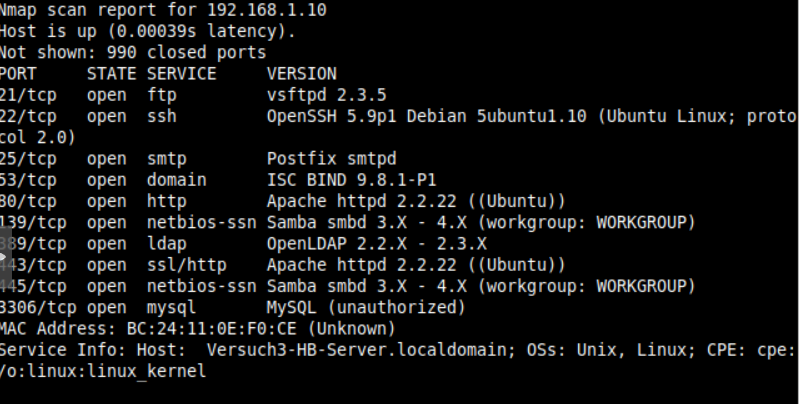
\includegraphics[width=0.7\textwidth]{img/Heartbleed/Portchec.png}
\caption{Nmap-Scan}
\label{fig:nmapscan}
\end{figure}
Wie in Abbildung \ref{fig:nmapscan} zu sehen ist, haben wir die IP-Adresse 192.168.1.10 des Servers gefunden. Nun nutzen wir Metasploit, das diesen Heartbleed-Angriff implementiert hat.\\
Wir verwenden dazu das Modul:

\begin{verbatim}
use auxiliary/scanner/ssl/openssl_heartbleed
\end{verbatim}

Zusätzlich setzen wir, wie in Abbildung \ref{fig:settingsMetaasploit} zu erkennen ist, folgende Parameter:

\begin{figure}[H]
\raggedright
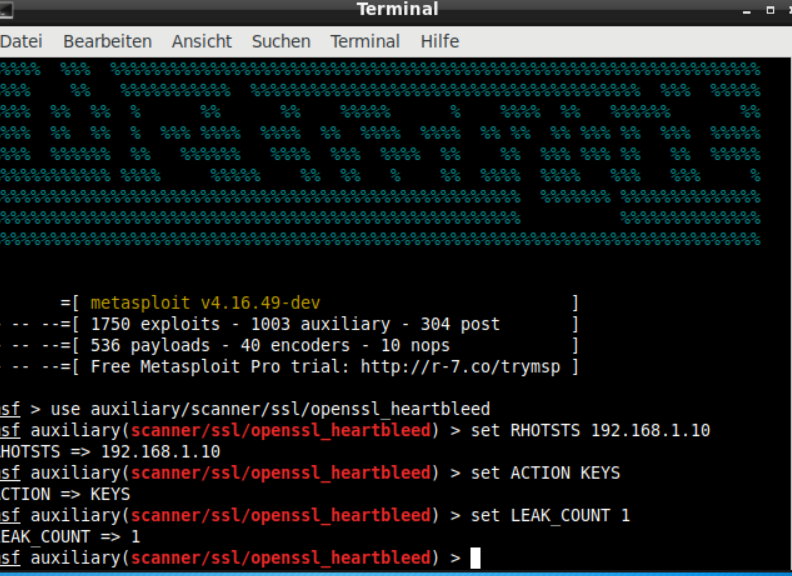
\includegraphics[width=0.5\textwidth]{img/Heartbleed/Settings_metasploit.png}
\caption{Metasploit-Einstellungen}
\label{fig:settingsMetaasploit}
\end{figure}

Wir haben \texttt{RHOSTS} gesetzt, ebenso eingestellt, dass nach einem Key gesucht wird und einmal Speicher angefordert wird.\\
Der Angriff war erfolgreich und wir haben den privaten Schlüssel erhalten:

\begin{figure}[H]
\raggedright
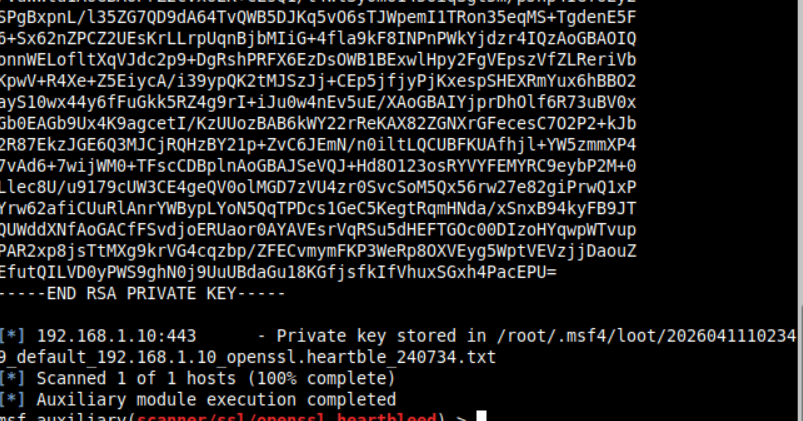
\includegraphics[width=0.5\textwidth]{img/Heartbleed/RSA_key_found.png}
\caption{RSA-Key gefunden}
\label{fig:RSA_KeyFound}
\end{figure}

Nun betrachten wir den Schlüssel, den wir erhalten haben, mit OpenSSL, um den Entschlüsselungsexponenten auszulesen:

\begin{verbatim}
openssl rsa -in /PFADzumSchlüsselAusA -text -noout
\end{verbatim}

\begin{figure}[H]
\raggedright
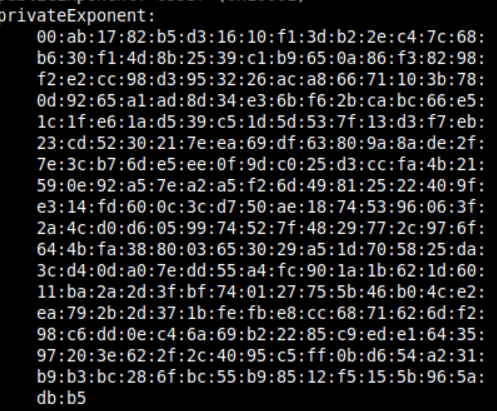
\includegraphics[width=0.5\textwidth]{img/Heartbleed/private_Exponent.png}
\caption{Entschlüsselungsexponent}
\label{fig:privateExponent}
\end{figure}

Das nächste Ziel ist nun, sich auf dem Server einzuloggen. Wir zeichnen dafür den Login des Clients am Server mit Wireshark auf.\\
Gleichzeitig konfigurieren wir, dass der Schlüssel, den wir zuvor erhalten haben, benutzt wird, um verschlüsselte Pakete zu entschlüsseln.

\begin{verbatim}
Wireshark -> Bearbeiten -> Protocols -> SSL suchen -> RSA key List [Edit] drücken
\end{verbatim}

Dann suchen wir das Paket, bei dem Inhalte vom Server angefragt wurden. Dieses Paket konnten wir anschließend mitlesen.

\begin{figure}[H]
\raggedright
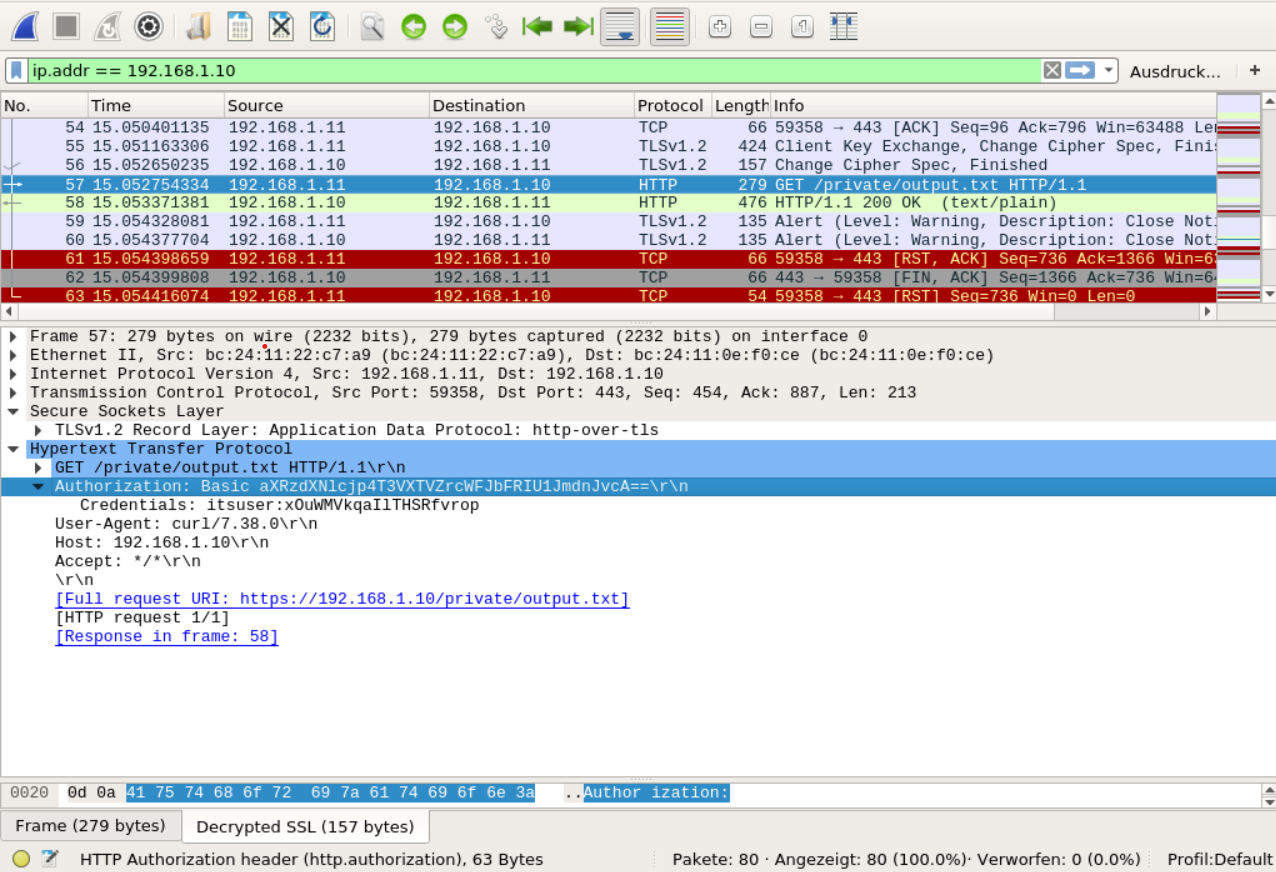
\includegraphics[width=0.5\textwidth]{img/Heartbleed/Wireshark_mitcredentials.png}
\caption{Wireshark mit Credentials}
\label{fig:Wireshark}
\end{figure}

Dadurch haben wir auch die Credentials erhalten, mit denen sich am Server angemeldet werden konnte. Ebenso konnte die angeforderte Datei abgegriffen werden.

\begin{figure}[H]
\raggedright
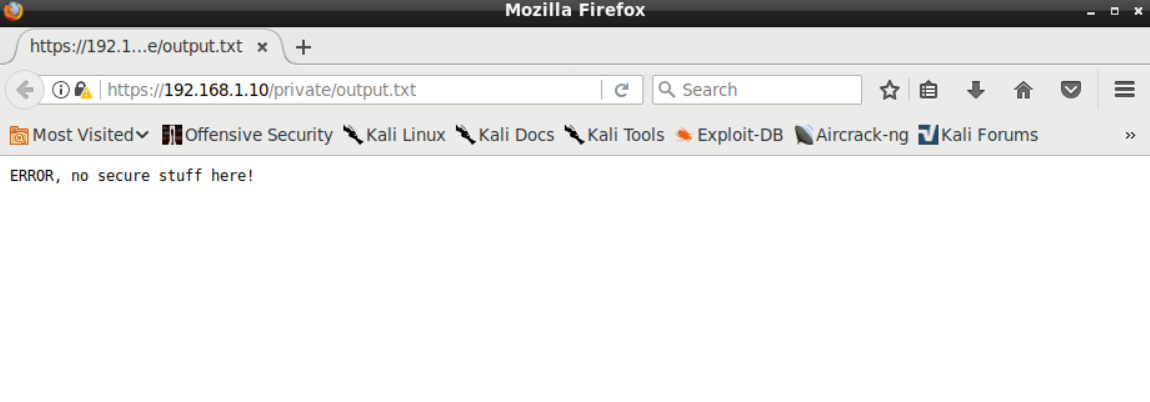
\includegraphics[width=0.7\textwidth]{img/Heartbleed/Eingeloggt_Outputtxt.png}
\caption{Output-Datei}
\label{fig:OutputTxt}
\end{figure}

\subsection{Wie ändert sich die Situation, wenn TLS mit DHE-RSA-Schlüsselaustausch anstelle von SSL mit RSA-Schlüsselaustausch bei gleichbleibendem RSA-Schlüssel verwendet wird?}
Beim klassischen RSA-Schlüsselaustausch wird der Sitzungsschlüssel direkt mit dem öffentlichen RSA-Schlüssel des Servers verschlüsselt. Schafft es ein Angreifer später den privaten RSA-Schlüssel durch z.B Heartbleed zu erlangen, können aufgezeichnetet Verbindungen nachträglich entschlüsselt werden\\
Beim DHE-RSA-Schlüsselaustausch hingegen wird der Sitzungsschlüssel mittels eines ephemeren Diffie-Hellman-Verfahrens ausgehandelt. Der RSA-Schlüssel dient hier nur zum Signieren des Schlüsselaustauschs, nicht zur direkten Verschlüsselung des Sitzungsschlüssels.
Also wenn der RSA-Schlüssel kompromitiert wird, kann dieser nicht mehr verwendet werden zum Entschlüsseln alter mitgeschnittener Verbindungen, da die Sitzungsschlüssel per ephemerem Diffie-Hellman erzeugt werden (Forward Secrecy). Wird jedoch Heartbleed aktiv gegen den laufenden Server ausgenutzt, können aktuelle Session Keys immernoch aus dem RAM ausgelesen werden. Dadurch lassen sich laufende oder kürzlich aufgezeichnete Sitzungen trotzdem entschlüsseln.
